\documentclass[11pt]{ctexart}
% Shared preamble of the v4 papers (Chinese; xelatex with ctex).
\usepackage[margin=1in]{geometry}
\usepackage{amsmath,amssymb}
\usepackage{booktabs,multirow,array}
\usepackage{graphicx}
\usepackage[font=small,labelfont=bf]{caption}
\usepackage{subcaption}
\usepackage{xcolor}
\usepackage{enumitem}
\usepackage[numbers,sort&compress]{natbib}
\usepackage[hidelinks]{hyperref}
\usepackage{url}
\setlist{nosep,leftmargin=*}
\newcommand{\kev}{Kev-4B}
\newcommand{\pc}{P_{\mathrm{c}}}
\newcommand{\pg}{P_{\mathrm{g}}}
\newcommand{\ci}[2]{[#1,\,#2]}
\newenvironment{correction}{\begin{center}\begin{minipage}{0.95\linewidth}\small\setlength{\parskip}{3pt}\noindent\textbf{更正声明。}}{\end{minipage}\end{center}}

% \NUM{key}: a number computed by dcjev/analysis/paper_numbers.py and written to the paper's numbers.tex.
% A key that numbers.tex does not define prints as ??key?? and logs a warning, so a missing number cannot vanish.
\makeatletter
\newcommand{\NUM}[1]{\ifcsname num@#1\endcsname\csname num@#1\endcsname\else\textbf{??\detokenize{#1}??}\PackageWarning{numbers}{Undefined number #1}\fi}
\newcommand{\defnum}[2]{\expandafter\def\csname num@#1\endcsname{#2}}
\makeatother

% Generated by dcjev/analysis/paper_numbers.py -- do not edit.
\defnum{cgall_hidden_he}{77.0}
\defnum{cgall_hidden_he_s1}{77.0}
\defnum{cgall_hidden_he_s2}{77.0}
\defnum{cgall_hidden_kod}{87.2}
\defnum{cgall_hidden_kod_s1}{86.6}
\defnum{cgall_hidden_kod_s2}{87.9}
\defnum{cgall_hidden_mbpp}{68.8}
\defnum{cgall_hidden_mbpp_s1}{68.6}
\defnum{cgall_hidden_mbpp_s2}{68.9}
\defnum{cgall_vis_he}{76.4}
\defnum{cgall_vis_he_s1}{77.6}
\defnum{cgall_vis_he_s2}{75.2}
\defnum{cgall_vis_kod}{86.6}
\defnum{cgall_vis_kod_s1}{86.2}
\defnum{cgall_vis_kod_s2}{86.9}
\defnum{cgall_vis_mbpp}{69.3}
\defnum{cgall_vis_mbpp_s1}{69.1}
\defnum{cgall_vis_mbpp_s2}{69.4}
\defnum{cgall_viskev_he}{76.7}
\defnum{cgall_viskev_he_s1}{77.6}
\defnum{cgall_viskev_he_s2}{75.8}
\defnum{cgall_viskev_kod}{86.6}
\defnum{cgall_viskev_kod_s1}{88.6}
\defnum{cgall_viskev_kod_s2}{84.6}
\defnum{cgall_viskev_mbpp}{72.3}
\defnum{cgall_viskev_mbpp_s1}{75.8}
\defnum{cgall_viskev_mbpp_s2}{68.9}
\defnum{cgallsd_hidden_he}{0.0}
\defnum{cgallsd_hidden_kod}{0.9}
\defnum{cgallsd_hidden_mbpp}{0.2}
\defnum{cgallsd_vis_he}{1.8}
\defnum{cgallsd_vis_kod}{0.5}
\defnum{cgallsd_vis_mbpp}{0.2}
\defnum{cgallsd_viskev_he}{1.3}
\defnum{cgallsd_viskev_kod}{2.8}
\defnum{cgallsd_viskev_mbpp}{4.9}
\defnum{cgatt_hidden_he}{1.29}
\defnum{cgatt_hidden_he_s1}{1.30}
\defnum{cgatt_hidden_he_s2}{1.27}
\defnum{cgatt_hidden_kod}{1.09}
\defnum{cgatt_hidden_kod_s1}{1.10}
\defnum{cgatt_hidden_kod_s2}{1.09}
\defnum{cgatt_hidden_mbpp}{1.41}
\defnum{cgatt_hidden_mbpp_s1}{1.41}
\defnum{cgatt_hidden_mbpp_s2}{1.40}
\defnum{cgatt_vis_he}{1.28}
\defnum{cgatt_vis_he_s1}{1.26}
\defnum{cgatt_vis_he_s2}{1.29}
\defnum{cgatt_vis_kod}{1.08}
\defnum{cgatt_vis_kod_s1}{1.09}
\defnum{cgatt_vis_kod_s2}{1.06}
\defnum{cgatt_vis_mbpp}{1.37}
\defnum{cgatt_vis_mbpp_s1}{1.36}
\defnum{cgatt_vis_mbpp_s2}{1.37}
\defnum{cgatt_viskev_he}{1.29}
\defnum{cgatt_viskev_he_s1}{1.27}
\defnum{cgatt_viskev_he_s2}{1.30}
\defnum{cgatt_viskev_kod}{1.11}
\defnum{cgatt_viskev_kod_s1}{1.08}
\defnum{cgatt_viskev_kod_s2}{1.13}
\defnum{cgatt_viskev_mbpp}{1.37}
\defnum{cgatt_viskev_mbpp_s1}{1.33}
\defnum{cgatt_viskev_mbpp_s2}{1.41}
\defnum{cgattsd_hidden_he}{0.02}
\defnum{cgattsd_hidden_kod}{0.01}
\defnum{cgattsd_hidden_mbpp}{0.01}
\defnum{cgattsd_vis_he}{0.02}
\defnum{cgattsd_vis_kod}{0.02}
\defnum{cgattsd_vis_mbpp}{0.01}
\defnum{cgattsd_viskev_he}{0.02}
\defnum{cgattsd_viskev_kod}{0.04}
\defnum{cgattsd_viskev_mbpp}{0.06}
\defnum{cgdall_hidden_he}{$+$0.6}
\defnum{cgdall_hidden_kod}{$+$0.7}
\defnum{cgdall_hidden_mbpp}{$-$0.5}
\defnum{cgdall_viskev_he}{$+$0.3}
\defnum{cgdall_viskev_kod}{$+$0.0}
\defnum{cgdall_viskev_mbpp}{$+$3.1}
\defnum{cgdallhi_hidden_he}{5.0}
\defnum{cgdallhi_hidden_kod}{3.2}
\defnum{cgdallhi_hidden_mbpp}{1.3}
\defnum{cgdallhi_viskev_he}{4.3}
\defnum{cgdallhi_viskev_kod}{2.5}
\defnum{cgdallhi_viskev_mbpp}{5.2}
\defnum{cgdalllo_hidden_he}{$-$3.4}
\defnum{cgdalllo_hidden_kod}{$-$1.8}
\defnum{cgdalllo_hidden_mbpp}{$-$2.5}
\defnum{cgdalllo_viskev_he}{$-$3.7}
\defnum{cgdalllo_viskev_kod}{$-$2.5}
\defnum{cgdalllo_viskev_mbpp}{1.1}
\defnum{cgdhack_hidden_he}{$-$0.9}
\defnum{cgdhack_hidden_kod}{$-$1.5}
\defnum{cgdhack_hidden_mbpp}{$-$2.1}
\defnum{cgdhack_viskev_he}{$-$0.9}
\defnum{cgdhack_viskev_kod}{$-$0.5}
\defnum{cgdhack_viskev_mbpp}{$-$2.5}
\defnum{cgdhackhi_hidden_he}{2.8}
\defnum{cgdhackhi_hidden_kod}{0.8}
\defnum{cgdhackhi_hidden_mbpp}{$-$0.3}
\defnum{cgdhackhi_viskev_he}{1.9}
\defnum{cgdhackhi_viskev_kod}{1.7}
\defnum{cgdhackhi_viskev_mbpp}{$-$0.7}
\defnum{cgdhacklo_hidden_he}{$-$4.7}
\defnum{cgdhacklo_hidden_kod}{$-$3.9}
\defnum{cgdhacklo_hidden_mbpp}{$-$4.0}
\defnum{cgdhacklo_viskev_he}{$-$3.7}
\defnum{cgdhacklo_viskev_kod}{$-$2.9}
\defnum{cgdhacklo_viskev_mbpp}{$-$4.5}
\defnum{cgfirst_hidden_he}{73.0}
\defnum{cgfirst_hidden_he_s1}{72.7}
\defnum{cgfirst_hidden_he_s2}{73.3}
\defnum{cgfirst_hidden_kod}{86.2}
\defnum{cgfirst_hidden_kod_s1}{85.6}
\defnum{cgfirst_hidden_kod_s2}{86.9}
\defnum{cgfirst_hidden_mbpp}{65.4}
\defnum{cgfirst_hidden_mbpp_s1}{65.7}
\defnum{cgfirst_hidden_mbpp_s2}{65.2}
\defnum{cgfirst_vis_he}{72.7}
\defnum{cgfirst_vis_he_s1}{74.5}
\defnum{cgfirst_vis_he_s2}{70.8}
\defnum{cgfirst_vis_kod}{84.7}
\defnum{cgfirst_vis_kod_s1}{84.6}
\defnum{cgfirst_vis_kod_s2}{84.9}
\defnum{cgfirst_vis_mbpp}{66.1}
\defnum{cgfirst_vis_mbpp_s1}{66.2}
\defnum{cgfirst_vis_mbpp_s2}{66.0}
\defnum{cgfirst_viskev_he}{73.3}
\defnum{cgfirst_viskev_he_s1}{73.3}
\defnum{cgfirst_viskev_he_s2}{73.3}
\defnum{cgfirst_viskev_kod}{83.9}
\defnum{cgfirst_viskev_kod_s1}{85.6}
\defnum{cgfirst_viskev_kod_s2}{82.2}
\defnum{cgfirst_viskev_mbpp}{68.0}
\defnum{cgfirst_viskev_mbpp_s1}{71.3}
\defnum{cgfirst_viskev_mbpp_s2}{64.6}
\defnum{cgfirstsd_hidden_he}{0.4}
\defnum{cgfirstsd_hidden_kod}{0.9}
\defnum{cgfirstsd_hidden_mbpp}{0.4}
\defnum{cgfirstsd_vis_he}{2.6}
\defnum{cgfirstsd_vis_kod}{0.2}
\defnum{cgfirstsd_vis_mbpp}{0.2}
\defnum{cgfirstsd_viskev_he}{0.0}
\defnum{cgfirstsd_viskev_kod}{2.4}
\defnum{cgfirstsd_viskev_mbpp}{4.7}
\defnum{cghack_hidden_he}{11.2}
\defnum{cghack_hidden_he_s1}{10.6}
\defnum{cghack_hidden_he_s2}{11.8}
\defnum{cghack_hidden_kod}{9.1}
\defnum{cghack_hidden_kod_s1}{9.1}
\defnum{cghack_hidden_kod_s2}{9.1}
\defnum{cghack_hidden_mbpp}{13.3}
\defnum{cghack_hidden_mbpp_s1}{13.0}
\defnum{cghack_hidden_mbpp_s2}{13.6}
\defnum{cghack_vis_he}{12.1}
\defnum{cghack_vis_he_s1}{11.2}
\defnum{cghack_vis_he_s2}{13.0}
\defnum{cghack_vis_kod}{10.6}
\defnum{cghack_vis_kod_s1}{10.1}
\defnum{cghack_vis_kod_s2}{11.1}
\defnum{cghack_vis_mbpp}{15.4}
\defnum{cghack_vis_mbpp_s1}{15.4}
\defnum{cghack_vis_mbpp_s2}{15.4}
\defnum{cghack_viskev_he}{11.2}
\defnum{cghack_viskev_he_s1}{11.2}
\defnum{cghack_viskev_he_s2}{11.2}
\defnum{cghack_viskev_kod}{10.1}
\defnum{cghack_viskev_kod_s1}{9.7}
\defnum{cghack_viskev_kod_s2}{10.4}
\defnum{cghack_viskev_mbpp}{12.9}
\defnum{cghack_viskev_mbpp_s1}{11.7}
\defnum{cghack_viskev_mbpp_s2}{14.1}
\defnum{cghacksd_hidden_he}{0.9}
\defnum{cghacksd_hidden_kod}{0.0}
\defnum{cghacksd_hidden_mbpp}{0.4}
\defnum{cghacksd_vis_he}{1.3}
\defnum{cghacksd_vis_kod}{0.7}
\defnum{cghacksd_vis_mbpp}{0.0}
\defnum{cghacksd_viskev_he}{0.0}
\defnum{cghacksd_viskev_kod}{0.5}
\defnum{cghacksd_viskev_mbpp}{1.7}
\defnum{cghackv_hidden_he}{12.7}
\defnum{cghackv_hidden_he_s1}{12.1}
\defnum{cghackv_hidden_he_s2}{13.3}
\defnum{cghackv_hidden_kod}{9.4}
\defnum{cghackv_hidden_kod_s1}{9.5}
\defnum{cghackv_hidden_kod_s2}{9.3}
\defnum{cghackv_hidden_mbpp}{16.2}
\defnum{cghackv_hidden_mbpp_s1}{16.0}
\defnum{cghackv_hidden_mbpp_s2}{16.5}
\defnum{cghackv_vis_he}{13.7}
\defnum{cghackv_vis_he_s1}{12.6}
\defnum{cghackv_vis_he_s2}{14.8}
\defnum{cghackv_vis_kod}{10.9}
\defnum{cghackv_vis_kod_s1}{10.5}
\defnum{cghackv_vis_kod_s2}{11.3}
\defnum{cghackv_vis_mbpp}{18.2}
\defnum{cghackv_vis_mbpp_s1}{18.2}
\defnum{cghackv_vis_mbpp_s2}{18.2}
\defnum{cghackv_viskev_he}{12.7}
\defnum{cghackv_viskev_he_s1}{12.6}
\defnum{cghackv_viskev_he_s2}{12.9}
\defnum{cghackv_viskev_kod}{10.4}
\defnum{cghackv_viskev_kod_s1}{9.9}
\defnum{cghackv_viskev_kod_s2}{11.0}
\defnum{cghackv_viskev_mbpp}{15.2}
\defnum{cghackv_viskev_mbpp_s1}{13.4}
\defnum{cghackv_viskev_mbpp_s2}{17.0}
\defnum{cghackvsd_hidden_he}{0.9}
\defnum{cghackvsd_hidden_kod}{0.1}
\defnum{cghackvsd_hidden_mbpp}{0.3}
\defnum{cghackvsd_vis_he}{1.6}
\defnum{cghackvsd_vis_kod}{0.6}
\defnum{cghackvsd_vis_mbpp}{0.0}
\defnum{cghackvsd_viskev_he}{0.2}
\defnum{cghackvsd_viskev_kod}{0.7}
\defnum{cghackvsd_viskev_mbpp}{2.6}
\defnum{cgseeds_hidden}{2}
\defnum{cgseeds_vis}{2}
\defnum{cgseeds_viskev}{2}
\defnum{cgszmax_he_allpass}{49.7}
\defnum{cgszmax_he_firstattemptallpass}{47.2}
\defnum{cgszmax_he_hack}{19.3}
\defnum{cgszmax_he_hackamongvispass}{28.2}
\defnum{cgszmax_he_vispass}{68.9}
\defnum{cgszmax_kod_allpass}{65.8}
\defnum{cgszmax_kod_firstattemptallpass}{60.4}
\defnum{cgszmax_kod_hack}{20.8}
\defnum{cgszmax_kod_hackamongvispass}{24.1}
\defnum{cgszmax_kod_vispass}{86.6}
\defnum{cgszmax_mbpp_allpass}{55.6}
\defnum{cgszmax_mbpp_firstattemptallpass}{50.3}
\defnum{cgszmax_mbpp_hack}{14.1}
\defnum{cgszmax_mbpp_hackamongvispass}{20.6}
\defnum{cgszmax_mbpp_vispass}{69.1}
\defnum{cgszmean_he_allpass}{49.1}
\defnum{cgszmean_he_firstattemptallpass}{46.6}
\defnum{cgszmean_he_hack}{18.8}
\defnum{cgszmean_he_hackamongvispass}{27.7}
\defnum{cgszmean_he_vispass}{67.9}
\defnum{cgszmean_kod_allpass}{65.5}
\defnum{cgszmean_kod_firstattemptallpass}{59.8}
\defnum{cgszmean_kod_hack}{20.4}
\defnum{cgszmean_kod_hackamongvispass}{23.7}
\defnum{cgszmean_kod_vispass}{85.9}
\defnum{cgszmean_mbpp_allpass}{54.8}
\defnum{cgszmean_mbpp_firstattemptallpass}{49.5}
\defnum{cgszmean_mbpp_hack}{13.7}
\defnum{cgszmean_mbpp_hackamongvispass}{20.0}
\defnum{cgszmean_mbpp_vispass}{68.6}
\defnum{cgszmin_he_allpass}{48.4}
\defnum{cgszmin_he_firstattemptallpass}{46.0}
\defnum{cgszmin_he_hack}{18.0}
\defnum{cgszmin_he_hackamongvispass}{26.9}
\defnum{cgszmin_he_vispass}{67.1}
\defnum{cgszmin_kod_allpass}{65.1}
\defnum{cgszmin_kod_firstattemptallpass}{59.4}
\defnum{cgszmin_kod_hack}{19.8}
\defnum{cgszmin_kod_hackamongvispass}{23.1}
\defnum{cgszmin_kod_vispass}{85.2}
\defnum{cgszmin_mbpp_allpass}{54.3}
\defnum{cgszmin_mbpp_firstattemptallpass}{48.9}
\defnum{cgszmin_mbpp_hack}{13.3}
\defnum{cgszmin_mbpp_hackamongvispass}{19.4}
\defnum{cgszmin_mbpp_vispass}{67.8}
\defnum{cgszruns_he_allpass}{6}
\defnum{cgszruns_he_firstattemptallpass}{6}
\defnum{cgszruns_he_hack}{6}
\defnum{cgszruns_he_hackamongvispass}{6}
\defnum{cgszruns_he_vispass}{6}
\defnum{cgszruns_kod_allpass}{6}
\defnum{cgszruns_kod_firstattemptallpass}{6}
\defnum{cgszruns_kod_hack}{6}
\defnum{cgszruns_kod_hackamongvispass}{6}
\defnum{cgszruns_kod_vispass}{6}
\defnum{cgszruns_mbpp_allpass}{6}
\defnum{cgszruns_mbpp_firstattemptallpass}{6}
\defnum{cgszruns_mbpp_hack}{6}
\defnum{cgszruns_mbpp_hackamongvispass}{6}
\defnum{cgszruns_mbpp_vispass}{6}
\defnum{cgszsd_he_allpass}{0.4}
\defnum{cgszsd_he_firstattemptallpass}{0.6}
\defnum{cgszsd_he_hack}{0.5}
\defnum{cgszsd_he_hackamongvispass}{0.5}
\defnum{cgszsd_he_vispass}{0.8}
\defnum{cgszsd_kod_allpass}{0.3}
\defnum{cgszsd_kod_firstattemptallpass}{0.4}
\defnum{cgszsd_kod_hack}{0.4}
\defnum{cgszsd_kod_hackamongvispass}{0.4}
\defnum{cgszsd_kod_vispass}{0.6}
\defnum{cgszsd_mbpp_allpass}{0.5}
\defnum{cgszsd_mbpp_firstattemptallpass}{0.5}
\defnum{cgszsd_mbpp_hack}{0.3}
\defnum{cgszsd_mbpp_hackamongvispass}{0.5}
\defnum{cgszsd_mbpp_vispass}{0.5}
\defnum{cgtrainallpass_hidden}{82.6}
\defnum{cgtrainallpass_vis}{79.7}
\defnum{cgtrainallpass_viskev}{81.9}
\defnum{cgtrainattemptsmean_hidden}{1.20}
\defnum{cgtrainattemptsmean_vis}{1.21}
\defnum{cgtrainattemptsmean_viskev}{1.18}
\defnum{cgtrainhack_hidden}{12.1}
\defnum{cgtrainhack_vis}{15.0}
\defnum{cgtrainhack_viskev}{13.7}
\defnum{cgtrainrewardmean_hidden}{82.6}
\defnum{cgtrainrewardmean_vis}{94.6}
\defnum{cgtrainrewardmean_viskev}{77.1}
\defnum{cgtrainvispass_hidden}{94.6}
\defnum{cgtrainvispass_vis}{94.6}
\defnum{cgtrainvispass_viskev}{95.6}
\defnum{cgvis_hidden_he}{88.2}
\defnum{cgvis_hidden_he_s1}{87.6}
\defnum{cgvis_hidden_he_s2}{88.8}
\defnum{cgvis_hidden_kod}{96.3}
\defnum{cgvis_hidden_kod_s1}{95.6}
\defnum{cgvis_hidden_kod_s2}{97.0}
\defnum{cgvis_hidden_mbpp}{82.0}
\defnum{cgvis_hidden_mbpp_s1}{81.6}
\defnum{cgvis_hidden_mbpp_s2}{82.4}
\defnum{cgvis_vis_he}{88.5}
\defnum{cgvis_vis_he_s1}{88.8}
\defnum{cgvis_vis_he_s2}{88.2}
\defnum{cgvis_vis_kod}{97.1}
\defnum{cgvis_vis_kod_s1}{96.3}
\defnum{cgvis_vis_kod_s2}{98.0}
\defnum{cgvis_vis_mbpp}{84.7}
\defnum{cgvis_vis_mbpp_s1}{84.6}
\defnum{cgvis_vis_mbpp_s2}{84.8}
\defnum{cgvis_viskev_he}{87.9}
\defnum{cgvis_viskev_he_s1}{88.8}
\defnum{cgvis_viskev_he_s2}{87.0}
\defnum{cgvis_viskev_kod}{96.6}
\defnum{cgvis_viskev_kod_s1}{98.3}
\defnum{cgvis_viskev_kod_s2}{95.0}
\defnum{cgvis_viskev_mbpp}{85.2}
\defnum{cgvis_viskev_mbpp_s1}{87.5}
\defnum{cgvis_viskev_mbpp_s2}{83.0}
\defnum{cgvissd_hidden_he}{0.9}
\defnum{cgvissd_hidden_kod}{0.9}
\defnum{cgvissd_hidden_mbpp}{0.6}
\defnum{cgvissd_vis_he}{0.4}
\defnum{cgvissd_vis_kod}{1.2}
\defnum{cgvissd_vis_mbpp}{0.2}
\defnum{cgvissd_viskev_he}{1.3}
\defnum{cgvissd_viskev_kod}{2.4}
\defnum{cgvissd_viskev_mbpp}{3.2}
\defnum{ch_elig_humanevalplus}{94\%}
\defnum{ch_elig_kodcodetrain}{77\%}
\defnum{ch_elig_kodcodeval}{78\%}
\defnum{ch_elig_mbppplus}{96\%}
\defnum{ch_finallpass_hidden}{4}
\defnum{ch_finallpass_vis}{2}
\defnum{ch_finallpass_viskev}{1}
\defnum{ch_finallpassn_hidden}{1285}
\defnum{ch_finallpassn_vis}{1283}
\defnum{ch_finallpassn_viskev}{1307}
\defnum{ch_finhack_hidden}{0}
\defnum{ch_finhack_vis}{1}
\defnum{ch_finhack_viskev}{0}
\defnum{ch_finhackn_hidden}{190}
\defnum{ch_finhackn_vis}{218}
\defnum{ch_finhackn_viskev}{193}
\defnum{ch_first_hidden}{0.2\%}
\defnum{ch_first_vis}{0.2\%}
\defnum{ch_first_viskev}{0.2\%}
\defnum{ch_hardcoded_copy}{488}
\defnum{ch_hardcoded_elig}{488}
\defnum{ch_hardcoded_frac}{96.3\%}
\defnum{ch_hardcoded_n}{507}
\defnum{ch_last_hidden}{0.0\%}
\defnum{ch_last_vis}{0.0\%}
\defnum{ch_last_viskev}{0.0\%}
\defnum{ch_max_hidden}{0.8\%}
\defnum{ch_max_vis}{0.7\%}
\defnum{ch_max_viskev}{0.7\%}
\defnum{ch_mean_hidden}{0.2\%}
\defnum{ch_mean_vis}{0.3\%}
\defnum{ch_mean_viskev}{0.3\%}
\defnum{ch_policyhack_copy}{2}
\defnum{ch_policyhack_elig}{199}
\defnum{ch_policyhack_frac}{0.8\%}
\defnum{ch_policyhack_n}{263}
\defnum{ch_policyother_copy}{34}
\defnum{ch_policyother_elig}{2777}
\defnum{ch_policyother_frac}{1.1\%}
\defnum{ch_policyother_n}{3{,}077}
\defnum{ch_reference_copy}{0}
\defnum{ch_reference_elig}{513}
\defnum{ch_reference_frac}{0.0\%}
\defnum{ch_reference_n}{537}
\defnum{cs_allpass_all}{14.0\%}
\defnum{cs_allpass_he}{12.3\%}
\defnum{cs_allpass_kod}{18.6\%}
\defnum{cs_allpass_mbpp}{11.2\%}
\defnum{cs_attempts_all}{3{,}340}
\defnum{cs_attempts_he}{644}
\defnum{cs_attempts_kod}{1{,}192}
\defnum{cs_attempts_mbpp}{1{,}504}
\defnum{cs_failn_all}{263}
\defnum{cs_failn_he}{37}
\defnum{cs_failn_kod}{169}
\defnum{cs_failn_mbpp}{57}
\defnum{cs_hack_all}{36\%}
\defnum{cs_hack_he}{32\%}
\defnum{cs_hack_kod}{43\%}
\defnum{cs_hack_mbpp}{25\%}
\defnum{cs_hardcoded}{507}
\defnum{cs_hardcoded_heldout}{1}
\defnum{cs_mixed_all}{62}
\defnum{cs_mixed_he}{7}
\defnum{cs_mixed_kod}{46}
\defnum{cs_mixed_mbpp}{9}
\defnum{cs_policy}{3{,}340}
\defnum{cs_problems_all}{442}
\defnum{cs_problems_he}{73}
\defnum{cs_problems_kod}{213}
\defnum{cs_problems_mbpp}{156}
\defnum{cs_reference}{537}
\defnum{cs_samples}{4}
\defnum{cs_visn_all}{732}
\defnum{cs_visn_he}{116}
\defnum{cs_visn_kod}{391}
\defnum{cs_visn_mbpp}{225}
\defnum{cs_vispass_all}{21.9\%}
\defnum{cs_vispass_he}{18.0\%}
\defnum{cs_vispass_kod}{32.8\%}
\defnum{cs_vispass_mbpp}{15.0\%}
\defnum{csauc_all_arc}{0.84}
\defnum{csauc_all_arg}{0.86}
\defnum{csauc_all_kevc}{0.87}
\defnum{csauc_all_kevg}{0.87}
\defnum{csauc_he_arc}{0.84}
\defnum{csauc_he_arg}{0.84}
\defnum{csauc_he_kevc}{0.86}
\defnum{csauc_he_kevg}{0.85}
\defnum{csauc_kod_arc}{0.87}
\defnum{csauc_kod_arg}{0.90}
\defnum{csauc_kod_kevc}{0.88}
\defnum{csauc_kod_kevg}{0.89}
\defnum{csauc_mbpp_arc}{0.74}
\defnum{csauc_mbpp_arg}{0.74}
\defnum{csauc_mbpp_kevc}{0.82}
\defnum{csauc_mbpp_kevg}{0.83}
\defnum{csaucall_all_arc}{0.93}
\defnum{csaucall_all_arg}{0.94}
\defnum{csaucall_all_kevc}{0.93}
\defnum{csaucall_all_kevg}{0.93}
\defnum{csaucall_he_arc}{0.97}
\defnum{csaucall_he_arg}{0.98}
\defnum{csaucall_he_kevc}{0.97}
\defnum{csaucall_he_kevg}{0.97}
\defnum{csaucall_kod_arc}{0.90}
\defnum{csaucall_kod_arg}{0.92}
\defnum{csaucall_kod_kevc}{0.89}
\defnum{csaucall_kod_kevg}{0.89}
\defnum{csaucall_mbpp_arc}{0.95}
\defnum{csaucall_mbpp_arg}{0.95}
\defnum{csaucall_mbpp_kevc}{0.95}
\defnum{csaucall_mbpp_kevg}{0.95}
\defnum{csaucallhi_all_arc}{0.94}
\defnum{csaucallhi_all_arg}{0.95}
\defnum{csaucallhi_all_kevc}{0.94}
\defnum{csaucallhi_all_kevg}{0.94}
\defnum{csaucallhi_he_arc}{0.99}
\defnum{csaucallhi_he_arg}{0.99}
\defnum{csaucallhi_he_kevc}{0.98}
\defnum{csaucallhi_he_kevg}{0.98}
\defnum{csaucallhi_kod_arc}{0.93}
\defnum{csaucallhi_kod_arg}{0.94}
\defnum{csaucallhi_kod_kevc}{0.91}
\defnum{csaucallhi_kod_kevg}{0.92}
\defnum{csaucallhi_mbpp_arc}{0.96}
\defnum{csaucallhi_mbpp_arg}{0.96}
\defnum{csaucallhi_mbpp_kevc}{0.96}
\defnum{csaucallhi_mbpp_kevg}{0.96}
\defnum{csaucalllo_all_arc}{0.92}
\defnum{csaucalllo_all_arg}{0.93}
\defnum{csaucalllo_all_kevc}{0.91}
\defnum{csaucalllo_all_kevg}{0.91}
\defnum{csaucalllo_he_arc}{0.96}
\defnum{csaucalllo_he_arg}{0.96}
\defnum{csaucalllo_he_kevc}{0.95}
\defnum{csaucalllo_he_kevg}{0.95}
\defnum{csaucalllo_kod_arc}{0.88}
\defnum{csaucalllo_kod_arg}{0.89}
\defnum{csaucalllo_kod_kevc}{0.86}
\defnum{csaucalllo_kod_kevg}{0.86}
\defnum{csaucalllo_mbpp_arc}{0.93}
\defnum{csaucalllo_mbpp_arg}{0.93}
\defnum{csaucalllo_mbpp_kevc}{0.93}
\defnum{csaucalllo_mbpp_kevg}{0.93}
\defnum{csauchi_all_arc}{0.87}
\defnum{csauchi_all_arg}{0.89}
\defnum{csauchi_all_kevc}{0.90}
\defnum{csauchi_all_kevg}{0.90}
\defnum{csauchi_he_arc}{0.92}
\defnum{csauchi_he_arg}{0.92}
\defnum{csauchi_he_kevc}{0.95}
\defnum{csauchi_he_kevg}{0.94}
\defnum{csauchi_kod_arc}{0.91}
\defnum{csauchi_kod_arg}{0.93}
\defnum{csauchi_kod_kevc}{0.92}
\defnum{csauchi_kod_kevg}{0.93}
\defnum{csauchi_mbpp_arc}{0.82}
\defnum{csauchi_mbpp_arg}{0.82}
\defnum{csauchi_mbpp_kevc}{0.89}
\defnum{csauchi_mbpp_kevg}{0.89}
\defnum{csauclo_all_arc}{0.81}
\defnum{csauclo_all_arg}{0.83}
\defnum{csauclo_all_kevc}{0.84}
\defnum{csauclo_all_kevg}{0.84}
\defnum{csauclo_he_arc}{0.75}
\defnum{csauclo_he_arg}{0.74}
\defnum{csauclo_he_kevc}{0.75}
\defnum{csauclo_he_kevg}{0.73}
\defnum{csauclo_kod_arc}{0.83}
\defnum{csauclo_kod_arg}{0.86}
\defnum{csauclo_kod_kevc}{0.84}
\defnum{csauclo_kod_kevg}{0.84}
\defnum{csauclo_mbpp_arc}{0.66}
\defnum{csauclo_mbpp_arg}{0.65}
\defnum{csauclo_mbpp_kevc}{0.75}
\defnum{csauclo_mbpp_kevg}{0.75}
\defnum{csaucw_all_arc}{0.81}
\defnum{csaucw_all_arg}{0.85}
\defnum{csaucw_all_kevc}{0.79}
\defnum{csaucw_all_kevg}{0.81}
\defnum{csaucw_he_arc}{0.79}
\defnum{csaucw_he_arg}{0.86}
\defnum{csaucw_he_kevc}{0.86}
\defnum{csaucw_he_kevg}{0.86}
\defnum{csaucw_kod_arc}{0.84}
\defnum{csaucw_kod_arg}{0.86}
\defnum{csaucw_kod_kevc}{0.78}
\defnum{csaucw_kod_kevg}{0.84}
\defnum{csaucw_mbpp_arc}{0.67}
\defnum{csaucw_mbpp_arg}{0.78}
\defnum{csaucw_mbpp_kevc}{0.78}
\defnum{csaucw_mbpp_kevg}{0.61}
\defnum{csaucwhi_all_arc}{0.90}
\defnum{csaucwhi_all_arg}{0.93}
\defnum{csaucwhi_all_kevc}{0.88}
\defnum{csaucwhi_all_kevg}{0.90}
\defnum{csaucwhi_he_arc}{1.00}
\defnum{csaucwhi_he_arg}{1.00}
\defnum{csaucwhi_he_kevc}{1.00}
\defnum{csaucwhi_he_kevg}{1.00}
\defnum{csaucwhi_kod_arc}{0.93}
\defnum{csaucwhi_kod_arg}{0.95}
\defnum{csaucwhi_kod_kevc}{0.89}
\defnum{csaucwhi_kod_kevg}{0.94}
\defnum{csaucwhi_mbpp_arc}{1.00}
\defnum{csaucwhi_mbpp_arg}{1.00}
\defnum{csaucwhi_mbpp_kevc}{1.00}
\defnum{csaucwhi_mbpp_kevg}{0.92}
\defnum{csaucwlo_all_arc}{0.71}
\defnum{csaucwlo_all_arg}{0.75}
\defnum{csaucwlo_all_kevc}{0.69}
\defnum{csaucwlo_all_kevg}{0.70}
\defnum{csaucwlo_he_arc}{0.50}
\defnum{csaucwlo_he_arg}{0.54}
\defnum{csaucwlo_he_kevc}{0.54}
\defnum{csaucwlo_he_kevg}{0.54}
\defnum{csaucwlo_kod_arc}{0.73}
\defnum{csaucwlo_kod_arg}{0.75}
\defnum{csaucwlo_kod_kevc}{0.67}
\defnum{csaucwlo_kod_kevg}{0.73}
\defnum{csaucwlo_mbpp_arc}{0.33}
\defnum{csaucwlo_mbpp_arg}{0.50}
\defnum{csaucwlo_mbpp_kevc}{0.50}
\defnum{csaucwlo_mbpp_kevg}{0.27}
\defnum{csd_all_kevcarc}{$+$0.030}
\defnum{csd_all_kevgarc}{$+$0.030}
\defnum{csd_all_kevgarg}{$+$0.013}
\defnum{csd_he_kevcarc}{$+$0.017}
\defnum{csd_he_kevgarc}{$+$0.005}
\defnum{csd_he_kevgarg}{$+$0.010}
\defnum{csd_kod_kevcarc}{$+$0.014}
\defnum{csd_kod_kevgarc}{$+$0.016}
\defnum{csd_kod_kevgarg}{$-$0.012}
\defnum{csd_mbpp_kevcarc}{$+$0.082}
\defnum{csd_mbpp_kevgarc}{$+$0.087}
\defnum{csd_mbpp_kevgarg}{$+$0.086}
\defnum{csdall_all_kevcarc}{$-$0.007}
\defnum{csdall_all_kevgarc}{$-$0.006}
\defnum{csdall_all_kevgarg}{$-$0.012}
\defnum{csdall_he_kevcarc}{$-$0.002}
\defnum{csdall_he_kevgarc}{$-$0.005}
\defnum{csdall_he_kevgarg}{$-$0.008}
\defnum{csdall_kod_kevcarc}{$-$0.017}
\defnum{csdall_kod_kevgarc}{$-$0.012}
\defnum{csdall_kod_kevgarg}{$-$0.024}
\defnum{csdall_mbpp_kevcarc}{$+$0.000}
\defnum{csdall_mbpp_kevgarc}{$-$0.003}
\defnum{csdall_mbpp_kevgarg}{$-$0.001}
\defnum{csdallhi_all_kevcarc}{0.002}
\defnum{csdallhi_all_kevgarc}{0.003}
\defnum{csdallhi_all_kevgarg}{$-$0.005}
\defnum{csdallhi_he_kevcarc}{0.009}
\defnum{csdallhi_he_kevgarc}{0.009}
\defnum{csdallhi_he_kevgarg}{0.002}
\defnum{csdallhi_kod_kevcarc}{$-$0.001}
\defnum{csdallhi_kod_kevgarc}{0.003}
\defnum{csdallhi_kod_kevgarg}{$-$0.011}
\defnum{csdallhi_mbpp_kevcarc}{0.009}
\defnum{csdallhi_mbpp_kevgarc}{0.007}
\defnum{csdallhi_mbpp_kevgarg}{0.008}
\defnum{csdalllo_all_kevcarc}{$-$0.017}
\defnum{csdalllo_all_kevgarc}{$-$0.015}
\defnum{csdalllo_all_kevgarg}{$-$0.020}
\defnum{csdalllo_he_kevcarc}{$-$0.015}
\defnum{csdalllo_he_kevgarc}{$-$0.019}
\defnum{csdalllo_he_kevgarg}{$-$0.020}
\defnum{csdalllo_kod_kevcarc}{$-$0.032}
\defnum{csdalllo_kod_kevgarc}{$-$0.028}
\defnum{csdalllo_kod_kevgarg}{$-$0.037}
\defnum{csdalllo_mbpp_kevcarc}{$-$0.008}
\defnum{csdalllo_mbpp_kevgarc}{$-$0.012}
\defnum{csdalllo_mbpp_kevgarg}{$-$0.009}
\defnum{csdhi_all_kevcarc}{0.050}
\defnum{csdhi_all_kevgarc}{0.052}
\defnum{csdhi_all_kevgarg}{0.033}
\defnum{csdhi_he_kevcarc}{0.087}
\defnum{csdhi_he_kevgarc}{0.076}
\defnum{csdhi_he_kevgarg}{0.069}
\defnum{csdhi_kod_kevcarc}{0.038}
\defnum{csdhi_kod_kevgarc}{0.043}
\defnum{csdhi_kod_kevgarg}{0.010}
\defnum{csdhi_mbpp_kevcarc}{0.124}
\defnum{csdhi_mbpp_kevgarc}{0.129}
\defnum{csdhi_mbpp_kevgarg}{0.128}
\defnum{csdlo_all_kevcarc}{0.011}
\defnum{csdlo_all_kevgarc}{0.007}
\defnum{csdlo_all_kevgarg}{$-$0.007}
\defnum{csdlo_he_kevcarc}{$-$0.052}
\defnum{csdlo_he_kevgarc}{$-$0.067}
\defnum{csdlo_he_kevgarg}{$-$0.054}
\defnum{csdlo_kod_kevcarc}{$-$0.008}
\defnum{csdlo_kod_kevgarc}{$-$0.010}
\defnum{csdlo_kod_kevgarg}{$-$0.038}
\defnum{csdlo_mbpp_kevcarc}{0.042}
\defnum{csdlo_mbpp_kevgarc}{0.046}
\defnum{csdlo_mbpp_kevgarg}{0.045}
\defnum{csdw_all_kevcarc}{$-$0.016}
\defnum{csdw_all_kevgarc}{$+$0.000}
\defnum{csdw_all_kevgarg}{$-$0.040}
\defnum{csdw_he_kevcarc}{$+$0.071}
\defnum{csdw_he_kevgarc}{$+$0.071}
\defnum{csdw_he_kevgarg}{$+$0.000}
\defnum{csdw_kod_kevcarc}{$-$0.054}
\defnum{csdw_kod_kevgarc}{$+$0.000}
\defnum{csdw_kod_kevgarg}{$-$0.022}
\defnum{csdw_mbpp_kevcarc}{$+$0.111}
\defnum{csdw_mbpp_kevgarc}{$-$0.056}
\defnum{csdw_mbpp_kevgarg}{$-$0.167}
\defnum{csdwhi_all_kevcarc}{0.053}
\defnum{csdwhi_all_kevgarc}{0.065}
\defnum{csdwhi_all_kevgarg}{0.021}
\defnum{csdwhi_he_kevcarc}{0.250}
\defnum{csdwhi_he_kevgarc}{0.250}
\defnum{csdwhi_he_kevgarg}{0.000}
\defnum{csdwhi_kod_kevcarc}{0.028}
\defnum{csdwhi_kod_kevgarc}{0.087}
\defnum{csdwhi_kod_kevgarg}{0.048}
\defnum{csdwhi_mbpp_kevcarc}{0.375}
\defnum{csdwhi_mbpp_kevgarc}{0.000}
\defnum{csdwhi_mbpp_kevgarg}{0.000}
\defnum{csdwlo_all_kevcarc}{$-$0.089}
\defnum{csdwlo_all_kevgarc}{$-$0.069}
\defnum{csdwlo_all_kevgarg}{$-$0.109}
\defnum{csdwlo_he_kevcarc}{0.000}
\defnum{csdwlo_he_kevgarc}{0.000}
\defnum{csdwlo_he_kevgarg}{0.000}
\defnum{csdwlo_kod_kevcarc}{$-$0.140}
\defnum{csdwlo_kod_kevgarc}{$-$0.089}
\defnum{csdwlo_kod_kevgarg}{$-$0.097}
\defnum{csdwlo_mbpp_kevcarc}{0.000}
\defnum{csdwlo_mbpp_kevgarc}{$-$0.200}
\defnum{csdwlo_mbpp_kevgarg}{$-$0.438}
\defnum{rh_above_arc}{0.8\%}
\defnum{rh_above_arg}{0.0\%}
\defnum{rh_above_kevc}{0.2\%}
\defnum{rh_above_kevg}{0.0\%}
\defnum{rh_auc_arc}{0.991}
\defnum{rh_auc_arg}{1.000}
\defnum{rh_auc_kevc}{0.997}
\defnum{rh_auc_kevg}{1.000}
\defnum{rh_hc_arc}{0.05}
\defnum{rh_hc_arg}{0.02}
\defnum{rh_hc_kevc}{0.07}
\defnum{rh_hc_kevg}{0.03}
\defnum{rh_problems}{507}
\defnum{rh_ref_arc}{0.79}
\defnum{rh_ref_arg}{0.80}
\defnum{rh_ref_kevc}{0.75}
\defnum{rh_ref_kevg}{0.75}


\title{可见测试、留出测试与评判模型：\\度量 GRPO 多轮代码修复中的奖励投机}
\author{DC-Jev-RL 项目，第三部分 A（第 4 版）}
\date{2026 年 10 月}

\begin{document}
\maketitle

\begin{correction}
本文第 1.0--3.0 版（“Agentic-Jev-GRPO”）已撤回，其结果并非由任何实验产生。产生这些结果的基准套件里没有任何加载、训练或评估模型的代码；每个准确率、学习曲线和消融结果都是写进脚本的数字。文中列出的基准（BFCL-v3、MBPP+、HumanEval+、SWE-bench-Verified-Mini）一个也没有运行。本版用实测实验运行 MBPP+ 和 HumanEval+，并去掉了工具调用和 SWE-bench 的说法。撤回的文件保存在仓库的 \texttt{withdrawn/} 目录下，\texttt{CORRECTION.md} 列出了错误之处。
\end{correction}

\begin{abstract}
% 第三部分 A：摘要（由 main_zh.tex 引入）。
用策略能看到的测试来奖励它，它可能学会满足这些测试，而不是解决问题。我们在多轮代码修复中测量这一点：Qwen3.5-4B-Base 写一个函数，看到第一个失败的示例测试后重写，最多三次；由留出测试判定最终程序是否正确。离线时，基座策略通过可见测试的尝试中有 \NUM{cs_hack_all} 在留出测试上失败；\kev{} 和一个同样大小的自回归评判模型都把这类尝试排在正确尝试之下（AUROC 分别为 \NUM{csauc_all_kevg} 和 \NUM{csauc_all_arg}），并且几乎完美地把对测试的硬编码查表程序与参考解答区分开。随后我们用 GRPO 训练 100 步，每种奖励两个种子：只用可见测试；可见测试乘以 \kev{} 对代码是否 genuine 的判断；以及作为预言机的全部测试。我们没有看到可见测试奖励被利用的迹象：解出题目的比例在 KodCode val（从 \NUM{cgszmean_kod_allpass}\% 升至 \NUM{cgall_vis_kod}\%）、MBPP+ 和 HumanEval+ 上都提高了，通过可见测试的程序中错误者的比例在三个集合中的两个上降低了约一半，抄写可见测试中数值的程序仍和基座策略中一样少见。评判因子带来的变化没有超出种子之间的差异；从不奖励错误程序的预言机奖励，让错误的通过略有减少，但没有解出更多题目。本版取代了结果并非由实验产生的早期版本。代码、日志和本文的每一个数字都在仓库中。

\end{abstract}

% 第三部分 A：引言与相关工作（由 main_zh.tex 引入）。

\section{引言}\label{sec:intro}

编程智能体通常只看到少量示例测试，而它写的代码必须在示例之外也能工作。用可见测试构造的训练奖励，奖励的是通过这些测试，而不是解决问题。策略可能学会以不能推广的方式满足示例，极端情况下直接对示例做特判。在以测试为奖励训练推理模型时，已经观察到这类奖励投机行为~\cite{baker2025monitoring,denison2024sycophancy,skalse2022defining}。

本文在一个小而完整的设定中测量评判模型能帮上多少忙。任务是多轮代码修复：策略写一个函数，看到第一个失败的示例测试及其报错，再试一次，最多三次。奖励有三种：只用可见测试；可见测试乘以 \kev{} 对代码是否“对所有合法输入都解决了问题，而不是对示例测试做特判”的判断；以及作为预言机的可见测试加留出测试。我们测量可见测试所证明的与留出测试所发现的之间的差距：离线地针对基座策略的代码和专为通过可见测试而构造的硬编码查表程序；在线地针对 GRPO 训练过程中和训练之后的策略。

\paragraph{更正。} 本文第 1--3 版（“Agentic-Jev-GRPO”）报告的 BFCL-v3、MBPP+、HumanEval+ 和 SWE-bench-Verified-Mini 结果并非由任何实验产生，“生成”这些结果的脚本里没有任何模型代码（见上方声明和 \file{CORRECTION.md}）。本版运行 MBPP+ 和 HumanEval+，并采用把每道题的测试划分为可见测试和留出测试的协议。本版不涉及工具调用基准和 SWE-bench。

\section{相关工作}\label{sec:related}

执行反馈是代码强化学习的标准奖励。EvalPlus~\cite{liu2023evalplus} 这类扩展了测试的基准表明，HumanEval 和 MBPP~\cite{chen2021codex,austin2021program} 的原始测试漏掉了许多错误程序，这正是只用可见测试的奖励所留下的缺口。KodCode~\cite{xu2025kodcode} 为强化学习提供带有已验证测试的合成题目。代码正确性的 LLM 评判，是第二部分在数学上研究的生成式验证器~\cite{zhang2024genverifier}在代码上的对应物。监控策略的推理以发现奖励投机迹象~\cite{baker2025monitoring}，是使用第二个模型的另一种方式；这里评判模型只读最终代码。

% 第三部分 A：不依赖结果的章节（由 main_zh.tex 引入）。

\section{任务：带可见测试和留出测试的代码修复}\label{sec:task}

\paragraph{题目。} 训练题来自 KodCode-Light-RL-10K~\cite{xu2025kodcode}：带 \texttt{pytest} 单元测试的 Python 函数题。我们保留这样的题目：测试文件只测一个函数，不使用 fixture 或第三方包，并且至少有三个测试函数。第一个测试函数展示给策略（\emph{可见}），其余的\emph{留出}。300 道题（种子 0）留作验证集（\texttt{kodcode\_val}）。测试集为 MBPP+ 和 HumanEval+~\cite{austin2021program,chen2021codex,liu2023evalplus}。MBPP+ 中原始 MBPP 的 assert 是可见的（多数题为三个，最多七个）；HumanEval+ 中原始 HumanEval 测试的前三个 assert 是可见的（原测试不足三个时取全部）。两者中，EvalPlus 测试框架及其新增的测试都是留出的。若一道题的参考解答在我们的测试框架下通不过它自己的任何测试，就丢弃该题，并报告丢弃数量。每个程序都在空临时目录中各自的 \texttt{python -I} 子进程里运行，限制 CPU 时间、地址空间和文件大小，并设墙钟超时；运行前禁用 \texttt{os}、\texttt{shutil} 和 \texttt{subprocess} 中的破坏性函数（即 OpenAI \texttt{human-eval} 的“reliability guard”）。这能约束小模型写出的有缺陷代码，但不是安全边界。

\paragraph{回合。} 策略看到题目、函数签名和可见测试，写出一个解答（每次尝试最多 768 个词元）。代码在可见测试上运行。若有测试失败，策略看到第一个失败的测试及其报错，再写一次，总共最多三次。每次尝试都接续之前各轮的完整词元序列。回合在第一次通过全部可见测试的尝试处结束，或在第三次尝试后结束，然后最终代码在留出测试上运行。提示见 \file{experiments/part3a_code/prompts/code_prompts.json}，在任何运行之前即已固定。

\paragraph{指标。} \emph{vis pass}：最终代码通过全部可见测试。\emph{all pass}：通过全部可见测试和全部留出测试。\emph{hack}：通过可见测试但有留出测试失败。它既统计过拟合或特判的解答，也统计仅仅是不完整的解答；这一指标无法区分两者，我们把它作为“可见测试所证明的”与“实际情况”之间的差距来报告。\emph{首次尝试 all pass} 衡量不经修复时策略的水平。

\section{奖励}\label{sec:rewards}

\begin{itemize}
\item \texttt{vis}：最终代码通过全部可见测试则为 1。这是只持有可见测试的智能体所能检查的全部内容，也正是诱发对可见测试过拟合的奖励。
\item \texttt{vis\_kev}：\texttt{vis} 乘以 \kev{} 对 \emph{genuine} 问题回答“是”的概率：“所给代码是否对所有合法输入都解决了问题，而不是对示例测试做特判？”\kev{} 看到题目、可见测试和最终代码，从不看到留出测试。
\item \texttt{hidden}：最终代码通过全部可见测试和全部留出测试则为 1。这是一个预言机：相当于测试完整时的 \texttt{vis}。
\end{itemize}
一个回合中的每次尝试都使用该回合的优势进行训练，反馈词元作为上下文，不参与训练。更新方式与第二部分相同：每题 8 个回合的组基线、批级尺度、词元级损失、截断重要性采样，每批一次优化器更新。

\section{离线评判研究}\label{sec:code-study}

训练之前，基座策略在 \texttt{kodcode\_val}、MBPP+ 和 HumanEval+ 上以温度 1 每题写 4 个单次尝试。我们在两组测试上运行它们，两个评判模型对每个尝试回答 \emph{genuine} 和 \emph{correct}。对可见测试奖励而言，关键问题是：在通过可见测试的尝试中，评判模型能否把同时通过留出测试的那些分出来。我们报告这一 AUROC，以及在全部尝试上识别“全部通过”的 AUROC。我们还为 MBPP+ 和 HumanEval+ 构造两类状态已知的代码：一类是参考解答；另一类是\emph{硬编码}查表程序，对每个可见测试的参数返回期望值，其他情况返回 \texttt{None}。查表程序只有在通过可见测试时才保留，因此它是纯粹对测试做特判的程序。我们报告每个评判模型给查表程序的分数高于同一道题参考解答的频率。

% 第三部分 A 结果：离线代码评判研究（由 main_zh.tex 引入）。

\section{评判模型在代码中看到了什么}\label{sec:res-study}

\paragraph{可见测试留下了很大的缺口。} 基座策略的 \NUM{cs_policy} 次单次尝试（每题 \NUM{cs_samples} 次）中，\NUM{cs_vispass_all} 通过可见测试，\NUM{cs_allpass_all} 通过全部测试。在通过可见测试的尝试中，\NUM{cs_hack_all} 有留出测试失败：KodCode val 上为 \NUM{cs_hack_kod}，MBPP+ 上为 \NUM{cs_hack_mbpp}，HumanEval+ 上为 \NUM{cs_hack_he}。在训练还没来得及利用它之前，用可见测试构造的奖励就已经给这些尝试与正确尝试同样多的奖励。

\paragraph{两个评判模型都能看出大部分问题，在训练分布上 \kev{} 并不更好。} 表~\ref{tab:code-study} 给出在通过可见测试的尝试中，各信号对“同时通过留出测试”的 AUROC。在三个数据集合并后，\kev{} 的 \emph{genuine} 达到 \NUM{csauc_all_kevg} \ci{\NUM{csauclo_all_kevg}}{\NUM{csauchi_all_kevg}}，AR 评判达到 \NUM{csauc_all_arg} \ci{\NUM{csauclo_all_arg}}{\NUM{csauchi_all_arg}}（按题目重采样得到的 95\% 区间）。两者之差 \NUM{csd_all_kevgarg} \ci{\NUM{csdlo_all_kevgarg}}{\NUM{csdhi_all_kevgarg}} 不能分辨。用 \emph{correct} 问题时，\kev{} 领先 \NUM{csd_all_kevcarc} \ci{\NUM{csdlo_all_kevcarc}}{\NUM{csdhi_all_kevcarc}}。两种差异的大部分都来自 MBPP+，在那里 \kev{} 的 \emph{genuine} 领先 \NUM{csd_mbpp_kevgarg} \ci{\NUM{csdlo_mbpp_kevgarg}}{\NUM{csdhi_mbpp_kevgarg}}。在策略训练所用的分布 KodCode val 上，AR 评判领先，但幅度不能分辨（\NUM{csd_kod_kevgarg} \ci{\NUM{csdlo_kod_kevgarg}}{\NUM{csdhi_kod_kevgarg}}）；在 HumanEval+ 上两者无法区分（\NUM{csd_he_kevgarg} \ci{\NUM{csdlo_he_kevgarg}}{\NUM{csdhi_he_kevgarg}}）。在全部尝试上，两个评判模型把全部通过的尝试与其余尝试区分得更好（\NUM{csaucall_all_kevg} 和 \NUM{csaucall_all_arg}），AR 评判略微领先（\NUM{csdall_all_kevgarg} \ci{\NUM{csdalllo_all_kevgarg}}{\NUM{csdallhi_all_kevgarg}}）。

\begin{table}[t]
\centering\small
\begin{tabularx}{\linewidth}{@{}>{\raggedright\arraybackslash}Xcccccc@{}}
\toprule
 & \multicolumn{5}{c}{held-out tests pass, among visible-pass attempts} & all pass \\ \cmidrule(lr){2-6}\cmidrule(l){7-7}
 & KodCode val & MBPP+ & HumanEval+ & all [95\% CI] & within & all \\ \midrule
attempts passing the visible tests & 391 & 225 & 116 & 732 & & \\
\quad of which fail a held-out test & 169 & 57 & 37 & 263 & & \\ \midrule
\kev{} \emph{genuine} & 0.89 & 0.83 & 0.85 & 0.87 \ci{0.84}{0.90} & 0.81 & 0.93 \\
\kev{} \emph{correct} & 0.88 & 0.82 & 0.86 & 0.87 \ci{0.84}{0.90} & 0.79 & 0.93 \\
AR \emph{genuine} & 0.90 & 0.74 & 0.84 & 0.86 \ci{0.83}{0.89} & 0.85 & 0.94 \\
AR \emph{correct} & 0.87 & 0.74 & 0.84 & 0.84 \ci{0.81}{0.87} & 0.81 & 0.93 \\
\bottomrule
\end{tabularx}

\caption{在基座策略通过可见测试的尝试中（每题 \NUM{cs_samples} 次尝试，温度 1），各评判信号对“通过留出测试”的 AUROC。\emph{within}：在 \NUM{cs_mixed_all} 道“通过可见测试的尝试中既有通过也有未通过留出测试者”的题目内部的平均 AUROC。\emph{all pass}：在全部尝试上识别“通过全部测试”的 AUROC。95\% 区间由按题目重采样得到。}
\label{tab:code-study}
\end{table}

\paragraph{题目内部的证据很少。} GRPO 的组基线比较的是同一道题的各个回合，所以 \texttt{vis\_kev} 中评判因子的作用，取决于它如何给一道题中通过可见测试的回合排序。在 \NUM{cs_problems_all} 道至少有一次尝试通过可见测试的题目中，只有 \NUM{cs_mixed_all} 道在留出测试上两种结果都有。在这些题目内部，\kev{} 的 \emph{genuine} 达到 \NUM{csaucw_all_kevg}，AR 评判达到 \NUM{csaucw_all_arg}，差值 \NUM{csdw_all_kevgarg} \ci{\NUM{csdwlo_all_kevgarg}}{\NUM{csdwhi_all_kevgarg}}。这些题目太少，既不足以给两个评判模型排序，也不足以预测评判因子会在多大程度上改变训练。

\paragraph{硬编码查表程序会被识破。} \NUM{cs_hardcoded} 个对可见测试调用做查表的程序通过了其所属 MBPP+ 或 HumanEval+ 题目的可见测试（其中 \NUM{cs_hardcoded_heldout} 个也通过了留出测试）。两个评判模型都几乎完美地把它们与同一批题目的参考解答区分开（表~\ref{tab:code-hardcoded}）。\kev{} 的 \emph{genuine} 给查表程序的平均分为 \NUM{rh_hc_kevg}，给参考解答的为 \NUM{rh_ref_kevg}，从未给查表程序打出高于其所属题目参考解答的分数。这类查表是对测试做特判最粗暴的方式。评判模型能识破它们，说明 \emph{genuine} 问题被正确理解了，但不能说明更隐蔽的过拟合也会被发现。

\begin{table}[t]
\centering\small
\begin{tabular}{@{}lcccc@{}}
\toprule
 & & \multicolumn{2}{c}{mean $p(\text{yes})$} & lookup scored \\ \cmidrule(lr){3-4}
signal & AUROC & reference & lookup & above reference \\ \midrule
\kev{} \emph{genuine} & 1.000 & 0.75 & 0.03 & 0.0\% \\
\kev{} \emph{correct} & 0.997 & 0.75 & 0.07 & 0.2\% \\
AR \emph{genuine} & 1.000 & 0.80 & 0.02 & 0.0\% \\
AR \emph{correct} & 0.991 & 0.79 & 0.05 & 0.8\% \\
\bottomrule
\end{tabular}

\caption{在 \NUM{rh_problems} 道可见测试允许构造查表程序的 MBPP+ 和 HumanEval+ 题目上，参考解答对硬编码查表程序：AUROC、两类程序的平均 $p(\text{yes})$，以及查表程序得分高于其所属题目参考解答的频率。}
\label{tab:code-hardcoded}
\end{table}

\paragraph{这预示着什么。} 评判因子可以压低通过可见测试却错误的尝试中的大部分，而 \kev{} 做到这一点的程度与 AR 评判——一个同样大小、被问同样问题的通用模型——相当。评判因子能否在训练中缩小这一差距，以及代价是多少可见测试通过率，要由训练实验来测量。

% 第三部分 A 结果：GRPO 训练（由 main_zh.tex 引入）。

\section{针对可见测试的训练}\label{sec:res-grpo}

每种奖励训练策略 100 步（每步 16 道题、每题 8 个回合，学习率 $10^{-5}$，与第二部分相同），各用 \NUM{cgseeds_vis} 个种子。表~\ref{tab:code-grpo} 给出最终策略在三个评估集上的结果，表~\ref{tab:code-paired} 给出奖励之间的配对差，图~\ref{fig:code-curves} 给出训练曲线。95\% 区间按题目重采样，不包含种子之间的差异，因此在种子结果不一致的地方，我们也给出每个种子的数值。

\paragraph{用可见测试训练让代码更正确。} 第 0 步时，基座策略在 \NUM{cgszmean_kod_allpass}\% 的 KodCode val 题目、\NUM{cgszmean_mbpp_allpass}\% 的 MBPP+ 题目和 \NUM{cgszmean_he_allpass}\% 的 HumanEval+ 题目上通过全部测试。用 \texttt{vis} 奖励训练 100 步后，这三个比例为 \NUM{cgall_vis_kod}\%、\NUM{cgall_vis_mbpp}\% 和 \NUM{cgall_vis_he}\%，而且需要的修复更少：它在首次尝试就解出 \NUM{cgfirst_vis_kod}\% 的 KodCode val 题目，第 0 步时为 \NUM{cgszmean_kod_firstattemptallpass}\%。MBPP+ 和 HumanEval+ 从未用于训练。

\paragraph{可见测试与留出测试之间的差距在两个集合上缩小了，在 MBPP+ 上没有。} 在基座策略于 KodCode val 上通过可见测试的尝试中，有 \NUM{cgszmean_kod_hackamongvispass}\% 在留出测试上失败；训练后为 \NUM{cghackv_vis_kod}\%。在 HumanEval+ 上，这一比例从 \NUM{cgszmean_he_hackamongvispass}\% 降到 \NUM{cghackv_vis_he}\%。在 MBPP+ 上它几乎不变，从 \NUM{cgszmean_mbpp_hackamongvispass}\% 到 \NUM{cghackv_vis_mbpp}\%：策略通过 MBPP+ 可见测试的题目多了很多（第 0 步为 \NUM{cgszmean_mbpp_vispass}\%，训练后为 \NUM{cgvis_vis_mbpp}\%），而可见测试通过、留出测试失败的题目占全部题目的比例从 \NUM{cgszmean_mbpp_hack}\% 增加到 \NUM{cghack_vis_mbpp}\%。训练没有让策略对可见测试的过拟合比基座策略更严重；但在 MBPP+ 上，也没有让它减轻。

\begin{table}[t]
\centering\small
\begin{tabular}{@{}lcccccccccc@{}}
\toprule
 & & \multicolumn{3}{c}{KodCode val} & \multicolumn{3}{c}{MBPP+} & \multicolumn{3}{c}{HumanEval+} \\ \cmidrule(lr){3-5}\cmidrule(lr){6-8}\cmidrule(lr){9-11}
condition & seeds & vis & all & hack & vis & all & hack & vis & all & hack \\ \midrule
\texttt{vis} & 2 & 97.1 & 86.6 & 10.6 & 84.7 & 69.3 & 15.4 & 88.5 & 76.4 & 12.1 \\
\texttt{vis\_kev} & 2 & 96.6 & 86.6 & 10.1 & 85.2 & 72.3 & 12.9 & 87.9 & 76.7 & 11.2 \\
\texttt{hidden} & 2 & 96.3 & 87.2 & 9.1 & 82.0 & 68.8 & 13.3 & 88.2 & 77.0 & 11.2 \\
\bottomrule
\end{tabular}

\caption{最终策略（贪心解码，最多三次尝试）：通过可见测试（\emph{vis}）、通过全部测试（\emph{all}），以及通过可见测试但有留出测试失败（\emph{hack}）的题目比例（\%）；种子均值。}
\label{tab:code-grpo}
\end{table}

\paragraph{预言机奖励：错误的通过略少，解出的题目没有增加。} \texttt{hidden} 只奖励通过全部测试的代码，因此从不奖励错误的程序。它的最终策略解出的题目与 \texttt{vis} 一样多：all pass 的差值在 KodCode val 上为 \NUM{cgdall_hidden_kod} \ci{\NUM{cgdalllo_hidden_kod}}{\NUM{cgdallhi_hidden_kod}} 个百分点，在 MBPP+ 上为 \NUM{cgdall_hidden_mbpp} \ci{\NUM{cgdalllo_hidden_mbpp}}{\NUM{cgdallhi_hidden_mbpp}}，在 HumanEval+ 上为 \NUM{cgdall_hidden_he} \ci{\NUM{cgdalllo_hidden_he}}{\NUM{cgdallhi_hidden_he}}（表~\ref{tab:code-paired}）。它通过可见测试的频率更低（MBPP+ 上为 \NUM{cgvis_hidden_mbpp}\%，\texttt{vis} 为 \NUM{cgvis_vis_mbpp}\%），而差异的大部分来自错误的程序：hack 率的差值分别为 \NUM{cgdhack_hidden_kod} \ci{\NUM{cgdhacklo_hidden_kod}}{\NUM{cgdhackhi_hidden_kod}}、\NUM{cgdhack_hidden_mbpp} \ci{\NUM{cgdhacklo_hidden_mbpp}}{\NUM{cgdhackhi_hidden_mbpp}} 和 \NUM{cgdhack_hidden_he} \ci{\NUM{cgdhacklo_hidden_he}}{\NUM{cgdhackhi_hidden_he}} 个百分点，只有在 MBPP+ 上区间不含零。
一个从不奖励错误程序的奖励，让其中一部分不再通过可见测试；但在 100 步之内，它没有把它们变成正确的程序。

\begin{table}[t]
\centering\small
\begin{tabular}{@{}lcccccc@{}}
\toprule
 & \multicolumn{3}{c}{all pass} & \multicolumn{3}{c}{hack} \\ \cmidrule(lr){2-4}\cmidrule(l){5-7}
minus \texttt{vis} & KodCode val & MBPP+ & HumanEval+ & KodCode val & MBPP+ & HumanEval+ \\ \midrule
\texttt{vis\_kev} & $+$0.0 & $+$3.1 & $+$0.3 & $-$0.5 & $-$2.5 & $-$0.9 \\
 & {\footnotesize \ci{$-$2.5}{2.5}} & {\footnotesize \ci{1.1}{5.2}} & {\footnotesize \ci{$-$3.7}{4.3}} & {\footnotesize \ci{$-$2.9}{1.7}} & {\footnotesize \ci{$-$4.5}{$-$0.7}} & {\footnotesize \ci{$-$3.7}{1.9}} \\[2pt]
\texttt{hidden} & $+$0.7 & $-$0.5 & $+$0.6 & $-$1.5 & $-$2.1 & $-$0.9 \\
 & {\footnotesize \ci{$-$1.8}{3.2}} & {\footnotesize \ci{$-$2.5}{1.3}} & {\footnotesize \ci{$-$3.4}{5.0}} & {\footnotesize \ci{$-$3.9}{0.8}} & {\footnotesize \ci{$-$4.0}{$-$0.3}} & {\footnotesize \ci{$-$4.7}{2.8}} \\[2pt]
\bottomrule
\end{tabular}

\caption{相对 \texttt{vis} 的配对差（百分点）：在每道题上取各条件的种子均值，求差后对题目取平均，并给出按题目重采样的 95\% 区间。}
\label{tab:code-paired}
\end{table}

\paragraph{评判因子：对 MBPP+ 的作用只出现在一个种子中。} \texttt{vis\_kev} 把可见测试奖励乘以 \kev{} 的 \emph{genuine} 分数。在 KodCode val 和 HumanEval+ 上，它的最终策略解出的题目与 \texttt{vis} 一样多（\NUM{cgdall_viskev_kod} \ci{\NUM{cgdalllo_viskev_kod}}{\NUM{cgdallhi_viskev_kod}} 和 \NUM{cgdall_viskev_he} \ci{\NUM{cgdalllo_viskev_he}}{\NUM{cgdallhi_viskev_he}}）。在 MBPP+ 上种子均值更好：all pass 的差值为 \NUM{cgdall_viskev_mbpp} \ci{\NUM{cgdalllo_viskev_mbpp}}{\NUM{cgdallhi_viskev_mbpp}} 个百分点，hack 率的差值为 \NUM{cgdhack_viskev_mbpp} \ci{\NUM{cgdhacklo_viskev_mbpp}}{\NUM{cgdhackhi_viskev_mbpp}}，按题目的区间不含零。但两个种子并不一致：\texttt{vis\_kev} 在种子 1 下通过 \NUM{cgall_viskev_mbpp_s1}\% 的 MBPP+ 题目的全部测试，在种子 2 下为 \NUM{cgall_viskev_mbpp_s2}\%，而 \texttt{vis} 分别为 \NUM{cgall_vis_mbpp_s1}\% 和 \NUM{cgall_vis_mbpp_s2}\%。两个种子中只有一个出现的效果，不是我们能够宣称的效果。

\paragraph{没有抄写测试。} hack 率统计每一个通过可见测试的错误程序，不论它只是不完整，还是对测试做了特判。为了区分两者，我们寻找最粗暴的特判形式：程序中出现了可见测试里的某个值（参数或期望结果），而参考解答中没有这个值（\file{dcjev/analysis/code_hacks.py}；只搜索被测函数及其用到的模块级代码，因此模型自己写的示例调用不算）。这项检查标出了离线研究中 \NUM{ch_hardcoded_n} 个硬编码查表程序中的 \NUM{ch_hardcoded_copy} 个，即每一个含有非平凡值的查表程序，而 \NUM{ch_reference_n} 个参考解答一个也没有标出。在离线研究中基座策略的尝试里，它标出了 \NUM{ch_policyhack_n} 个通过可见测试但有留出测试失败的尝试中的 \NUM{ch_policyhack_copy} 个，以及其余尝试的 \NUM{ch_policyother_frac}。训练期间，在 \texttt{vis} 的任何一个十步窗口中，它最多标出 \NUM{ch_max_vis} 的回合（\texttt{vis\_kev} 为 \NUM{ch_max_viskev}，\texttt{hidden} 为 \NUM{ch_max_hidden}），且没有上升趋势（表~\ref{tab:code-copies}）。在最终评估中，它标出了 \texttt{vis} 的 \NUM{ch_finhackn_vis} 个 hack 回合中的 \NUM{ch_finhack_vis} 个、\texttt{vis\_kev} 的 \NUM{ch_finhackn_viskev} 个中的 \NUM{ch_finhack_viskev} 个，以及 \texttt{hidden} 的 \NUM{ch_finhackn_hidden} 个中的 \NUM{ch_finhack_hidden} 个。通过可见测试的错误程序几乎从不含有测试中的值，训练前后都是如此；可见测试奖励没有教会策略抄写测试。不抄写任何值的特判，这项检查发现不了。

\begin{table}[t]
\centering\small
\begin{tabular}{@{}lcccccc@{}}
\toprule
 & & \multicolumn{3}{c}{training episodes that copy} & \multicolumn{2}{c}{final evaluation, copy} \\ \cmidrule(lr){3-5}\cmidrule(l){6-7}
condition & seeds & steps 0--9 & steps 50--59 & steps 90--99 & hack & all pass \\ \midrule
\texttt{vis} & 2 & 0.2\% & 0.2\% & 0.0\% & 1 / 218 & 2 / 1283 \\
\texttt{vis\_kev} & 2 & 0.2\% & 0.1\% & 0.0\% & 0 / 193 & 1 / 1307 \\
\texttt{hidden} & 2 & 0.2\% & 0.0\% & 0.0\% & 0 / 190 & 4 / 1285 \\
\bottomrule
\end{tabular}

\caption{含有参考解答中没有的可见测试值的程序：三个十步窗口中训练回合的比例（种子均值），以及最终评估的 hack 回合和 all pass 回合中的数量（所有种子和评估集合计）。}
\label{tab:code-copies}
\end{table}

\begin{figure}[t]
\centering
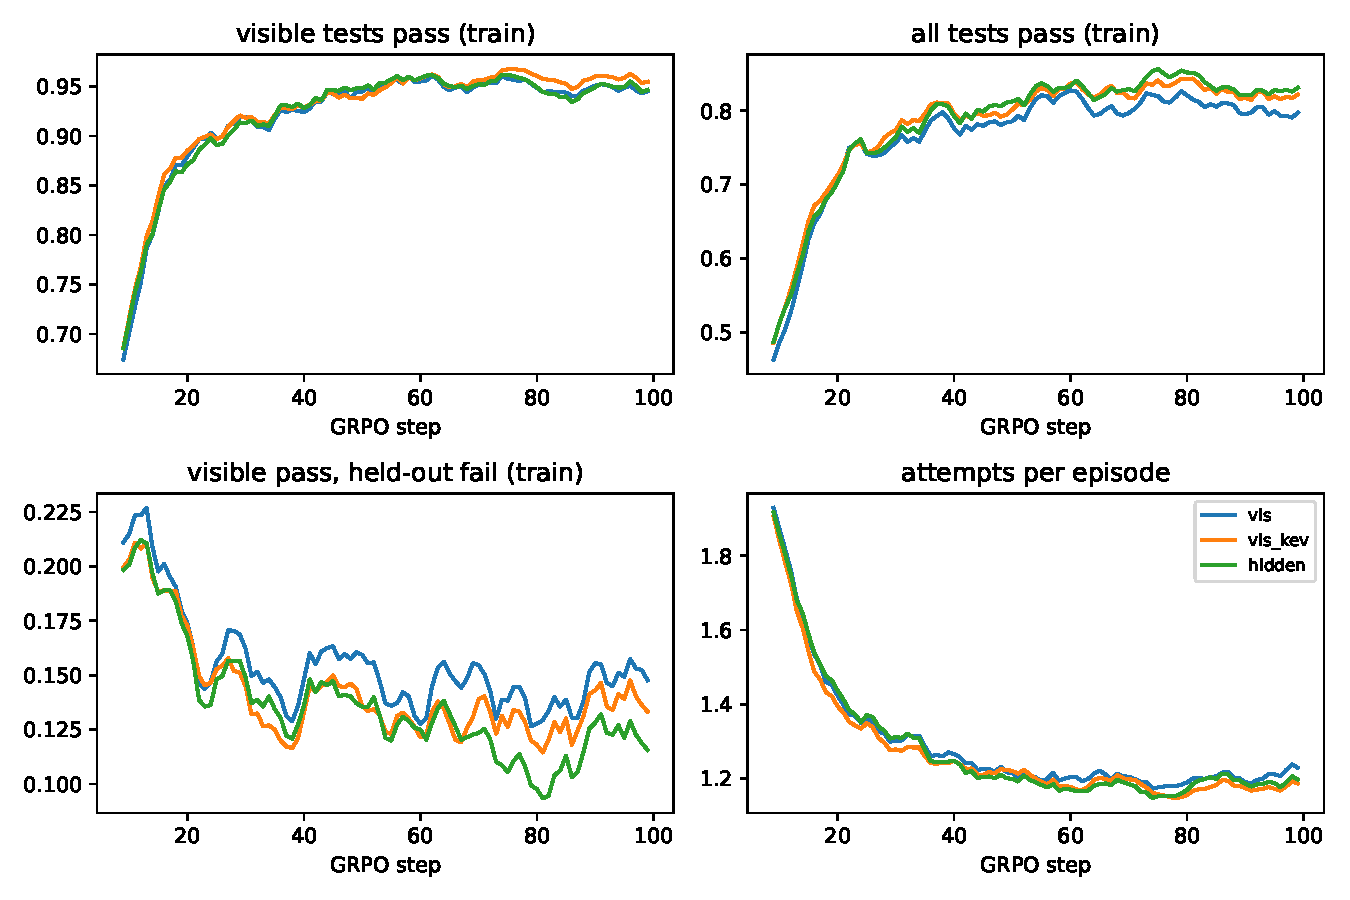
\includegraphics[width=\linewidth]{../../experiments/part3a_code/results/training_curves.pdf}
\caption{训练曲线（种子均值，10 步滑动平均）：训练回合中通过可见测试、通过全部测试、通过可见测试但有留出测试失败的比例，以及每个回合的尝试次数。}
\label{fig:code-curves}
\end{figure}

\paragraph{评估噪声。} 每次运行都在第 0 步评估同一个基座模型。在 \NUM{cgszruns_kod_allpass} 次运行中，KodCode val 上的 all pass 介于 \NUM{cgszmin_kod_allpass}\% 和 \NUM{cgszmax_kod_allpass}\% 之间（标准差 \NUM{cgszsd_kod_allpass} 个百分点），MBPP+ 上介于 \NUM{cgszmin_mbpp_allpass}\% 和 \NUM{cgszmax_mbpp_allpass}\% 之间，HumanEval+ 上介于 \NUM{cgszmin_he_allpass}\% 和 \NUM{cgszmax_he_allpass}\% 之间。vLLM 上的贪心解码在不同的服务器状态下不能逐位复现。同一奖励不同种子之间的差异更大：all pass 的标准差最高达 \NUM{cgallsd_viskev_mbpp} 个百分点（\texttt{vis\_kev}，MBPP+）。

% 第三部分 A：讨论（由 main_zh.tex 引入）。

\section{讨论}\label{sec:discussion}

\paragraph{没有看到可见测试被利用的迹象。} 本文关心的问题是：用策略能看到的测试来奖励它，它可能学会满足这些测试，而不是解决问题。在我们的设置中，100 步之内没有看到这种迹象。训练提高了三个集合上解出题目的比例，包括策略从未训练过的两个集合。通过可见测试的程序中错误者的比例，在 KodCode val 和 HumanEval+ 上降低了约一半，在 MBPP+ 上几乎不变。抄写可见测试中数值的程序，仍和基座策略中一样少见。通过可见测试的错误程序，在训练前后都几乎从不是对测试的抄写：它们处理了示例所展示的情况，却把其他情况做错了。可见测试奖励会奖励这些程序，但基座策略本来就会写出它们，而在三个集合中的两个上，训练让它们在通过者中所占的比例变小了。

\paragraph{评判模型能做什么，实际做了什么。} 离线时，两个评判模型给一道题中通过可见测试的尝试排序时，都能比随机更好地分出也通过留出测试的那些（\S\ref{sec:res-study}），而且都能识破硬编码查表程序。在训练中，评判因子带来的变化没有超出种子之间的差异：在 KodCode val 和 HumanEval+ 上没有差别，在 MBPP+ 上一个种子有提升，另一个没有。剩下需要压制的不是对测试的抄写，而是在示例未展示的情况上出错的解答。在策略确实学会特判的情形下——测试更弱、题目更难或训练更长——评判因子是否有用，这些运行无法回答。

\paragraph{更好的测试去掉的是少量错误的通过，而不是未解出的题目。} 预言机奖励只奖励通过全部测试的程序。它最终在三个集合上都让通过可见测试的错误程序比 \texttt{vis} 更少（只有在 MBPP+ 上区间不含零），而解出题目的比例相同。
在 100 步之内，知道哪些可见测试通过是错误的，并没有教会策略解出更多题目；它教会的是在解不出时更少地通过可见测试。一个对正确性完美的评判模型作为因子，给出的恰好就是这个奖励。

\paragraph{局限。} 只有一种策略规模（4B）、一种任务格式（单个函数，最多三次尝试，以第一个失败的测试作为反馈）、100 步、一个取自第二部分的学习率，以及每种奖励两个种子；在 MBPP+ 上两个种子的标准差高达 \NUM{cgallsd_viskev_mbpp} 个百分点。区间对题目重采样，不对种子重采样。留出测试是 KodCode 和 EvalPlus 的测试，一个程序通不过它们，是按它们的规格判定为错，而这种规格可能比题目描述更严格。特判检查只能发现含有可见测试中数值的程序；不含此类数值的特判（比如按输入长度分支）检测不到。训练期间其他实验共用 GPU。


\section*{可复现性}
代码、提示、数据准备（题目筛选和可见/留出测试的划分）、原始日志（每个 GRPO 步和最终评估的每个回合），以及离线研究的程序和评判分数都在仓库中（\texttt{experiments/part3a\_code/}）。表格和正文中的每个数字都由 \texttt{dcjev/code/judge\_study.py}、\texttt{dcjev/analysis/part3a.py} 和 \texttt{dcjev/analysis/paper\_numbers.py} 从中生成。

\bibliographystyle{plainnat}
\bibliography{../common/refs}
\end{document}
